\section{Advanced Optimization}

\subsection{The Problem of Poor Conditioning}

\begin{frame}{The Problem of Poor Conditioning}
    \frametitle{The Challenge of the Error Surface}
    \begin{itemize}
        \item The error surface of a neural network can have very different curvature along different directions.
        \item When the contours of the error surface are elongated ellipsoids, the problem is said to be \textbf{poorly conditioned} or \textbf{ill-conditioned}.
        \item This creates a scenario resembling a long, narrow valley.
    \end{itemize}
    \begin{figure}
        % Placeholder for the elongated ellipsoid visualization from Optimization I.pdf, p. 18
        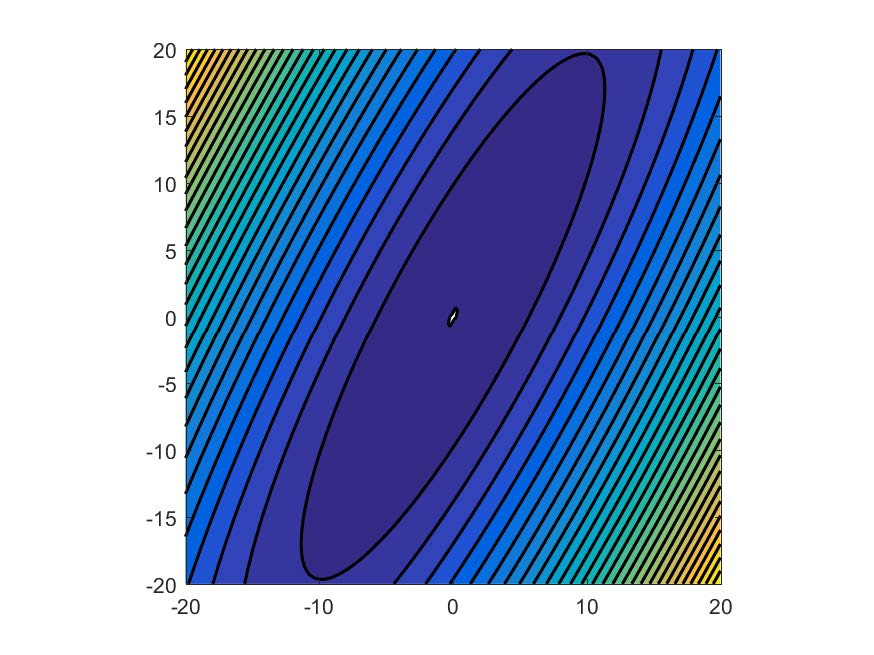
\includegraphics[width=0.5\textwidth]{images/elongated_ellipsoid.jpeg}
        \caption{An ill-conditioned error surface with elliptical contour lines.}
    \end{figure}
\end{frame}

\begin{frame}{Consequences of Poor Conditioning}
    \frametitle{Inefficient Gradient Descent}
    A single learning rate struggles on an ill-conditioned surface.
    \begin{itemize}
        \item The gradient vector is always perpendicular to the contour lines.
        \item In a narrow valley, this means the gradient points mostly across the valley, not along it.
        \item \textbf{Result:} The optimization path "zig-zags" inefficiently.
        \begin{itemize}
            \item \textbf{Fast oscillations} across the steep direction (the valley walls).
            \item \textbf{Slow progress} along the shallow direction (the valley floor).
        \end{itemize}
    \end{itemize}
    \begin{figure}
        % Placeholder for the oscillating gradient descent path from Optimization I.pdf, p. 18
        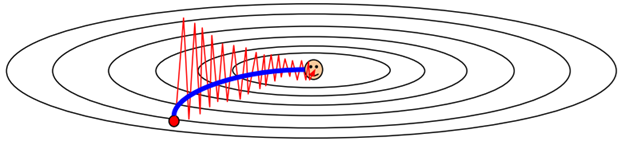
\includegraphics[width=1\textwidth]{images/zigzag.png}
        \caption{Gradient descent oscillates in the steep direction while making slow progress in the shallow direction.}
    \end{figure}
\end{frame}

\begin{frame}{The Learning Rate Dilemma}
    \frametitle{One Step Size, Two Different Needs}
    The core issue is that different directions require different optimal learning rates.
    \begin{itemize}
        \item To prevent divergence, the learning rate $\eta$ must be small enough for the steepest direction.
        \item This small learning rate is then far too small for the shallow direction, leading to extremely slow convergence.
        \item This conflict forces a compromise that is suboptimal for all directions.
    \end{itemize}
    \begin{alertblock}{The Motivation for Advanced Optimizers}
        Poor conditioning is a key reason that vanilla gradient descent is often too slow. This motivates methods that can adapt and take appropriately sized steps in different directions.
    \end{alertblock}
\end{frame}
